\chapter{Introducci\'on}
\label{cap:introduccion}

\section{Antecedentes y motivación}
\label{intro:motivacion}
% Hacer un prologo donde hable de la brecha entre lo real y lo virtual y como existen acercamientos que buscan minimizar su visibilidad/presencia
Según el continuo de la virtualidad de Milgram, la realidad mixta (MR del inglés \textit{mixed reality}) abarca todo tipo de enfoques que permiten combinar elementos virtuales con el mundo real. La realidad aumentada (AR, de \textit{augmented reality}) corresponde a uno de estos enfoques y, gracias a los avances tecnológicos en décadas recientes, este ha ganado terreno en distintas áreas como el turismo, el \textit{retail}, el cuidado médico, la industria, entre otras (\cite{jung_dieck_2018}).

Un caso puntual de la aplicación de AR corresponde a sistemas de ``lectura aumentada'', los cuales por medio del enfoque señalado son capaces de apoyar el proceso de lectura de documentos físicos, al facilitar ciertas tareas y, al mismo tiempo, otorgar acceso a utilidades a las que no se tiene acceso al momento de leer un libro o documento físico por si sólo, donde los límites del apoyo otorgado dependen únicamente de la tecnología empleada. 

EDDIE (\textit{Augment\textbf{ED} Rea\textbf{DI}ng D\textbf{E}ck}) es un tipo de sistema de lectura aumentada, resultado del trabajo conjunto entre alumnos y académicos del departamento de Ingeniería en Informática de la Universidad de Santiago de Chile. Este sistema, permite la interacción entre un lector y un documento sin la necesidad de usar dispositivos adicionales (como por ejemplo, smartphones y/o tablets), que puedan actuar como un obstáculo en una sesión de lectura.

%  need eddie pic here?

% Si bien eddie es un sistema que se encuentra en un estado funcional, existe la posibilidad de extender sus capacidades  al trabajar sobre cuatro de los distintos módulos que lo componen: interacciones, datos, consistencia, usabilidad. El trabajo sobre estos módulos permite por un lado, beneficios para lector, mientras que por otro lado, tambien abre las puertas para <beneficios quienes usan la plataforma para estudios>

% Acá usar un parrafo final para explicar cómo existe un tipo de tecnología que es perfecta para la labor principal de la plataforma (la lectura de docs), el seguimiento de movs oculares y porqué

\section{Descripci\'on del problema}
\label{intro:problema}
% 1. Problema surge del display utilizado en conjunto a la tecnología de eye tracking empleada
% 2. usualemnte este display corresponde a un monitor frente al usuario (confirmar esto)
% 3. sin embargo el display de la plataforma corresponde a un proyector, el cual proyecta (redundante?) una imagen sobre una mesa 
% 4. las diferencias que introduce trabajar con este tipo de display estan ligadas a la posición del usuario respecto a la imagen que observa y al nivel de luz generado por el display en sí, el cual puede interferir en las mediciones realizadas por el dispositivo eye tracking
% 5. Tomando en consideración estos dos tipos de display, ¿es posible integrar tecnologías de eye tracking sobre la plataforma, asegurando un nivel de precisión similar o equivalente al que se obtiene normalmente en monitores?

% * También el problema es determinar la forma en que se debe construir un plugin para que sea capaz de aceptar todo tipo de dispositivos de eye tracking, no solo limitandolo a los que se mencionan...

Debido a que el \textit{display} que utiliza la plataforma (correspondiente a un proyector) difiere de aquel empleado tradicionalmente con sensores \textit{eye tracking} (monitores), surgen dos desafíos por enfrentar:
\begin{enumerate}
    \item En primer lugar, se debe determinar dónde ubicar el sensor en la plataforma, tomando en consideración la ubicación del usuario y la luz generada por el proyector, ya que esta puede interferir en las mediciones realizadas por el sensor.
    \item En segundo lugar, se debe escoger un método de mapeo de movimientos oculares, de forma tal que se interprete de forma correcta aquello que el usuario observa en el documento y la proyección generada sobre él.
\end{enumerate}

Tomando en consideración estos desafíos mencionados, el problema que se planea abordar corresponde en cómo integrar tecnologías de rastreo de movimiento ocular sobre una plataforma que hace uso de una proyección como \textit{display}, de modo que se alcancen niveles de precisión similares o equivalentes a aquellos manejados en \textit{displays} tradicionales (monitores).

\section{Soluci\'on propuesta}
\label{intro:solucion}
\subsection{Características de la solución}
La solución, consiste en el desarrollo de un módulo de interacciones para habilitar el uso de tecnologías \textit{eye tracking} en la plataforma sobre la que se trabaja. Se busca que esta cumpla con los siguientes aspectos:
\begin{itemize}
    \item Permitir interacciones con la plataforma por medio de los movimientos oculares del usuario. %pensar qué tipo de interacciones son estas, no ahora, pero en caso de que pregunten en la presentación 
    \item Permitir el registro y almacenamiento de los movimientos oculares capturados, a modo de que estos datos se encuentren disponibles para ser manipulados.
    \item La solución debe hacer uso de un lenguaje de programación y un \textit{framework} definidos previamente, ya que se desarrolla sobre una plataforma ya existente.
\end{itemize}

\subsection{Propósito de la solución}
% Integrar tecnologías de eye tracking a la plataforma de lectura aumentada 
La solución se enfoca en dos de los cuatro aspectos en los que se pueden introducir mejoras: captura de datos e interacciones. Esta busca extender y reforzar las características del sistema de lectura aumentada no obstrusiva, al habilitar el uso de tecnologías que capturan datos desde movimientos oculares.

\section{Objetivos y alcance del proyecto}
\label{intro:objetivos}

\subsection{Objetivo general}
Ofrecer un módulo de interacciones basadas en movimientos oculares, para habilitar el correcto registro de dichos movimientos en una plataforma de lectura aumentada no obstrusiva, por medio de tecnologías de \textit{eye tracking} o seguimiento ocular.

\subsection{Objetivos espec\'ificos}
Para lograr el objetivo general, se plantean los siguientes objetivos específicos del trabajo:
\begin{enumerate}
    \item Levantar un estado del arte sobre los distintos métodos de mapeo (\textit{gaze mapping}) utilizados en la actualidad.
    \item Proveer de un método de \textit{gaze mapping} para rastrear movimientos oculares con el tipo de \textit{display} empleado por la plataforma.
    \item Diseñar una solución genérica, a modo de que no se limite al uso de un solo dispositivo de \textit{eye tracking}.
    \item Ejecutar pruebas para determinar la precisión con la que se rastrean los movimientos oculares.
\end{enumerate}

\subsection{Alcances y limitaciones}
\begin{itemize}
    \item La solución por ser implementada es genérica, esto significa, que por cada dispositivo \textit{eye tracker} que use un \textit{software development kit} (SDK) distinto, será posible crear una extensión que se conecta a la solución, sin la necesidad de implementar todo desde cero.
    \item La solución contempla como número de usuarios máximos concurrentes solo uno, por la naturaleza de la plataforma sobre la cual se trabaja.
    \item La posición donde se ubica el dispositivo de \textit{eye tracking} no podrá ser cambiada una vez determinada.
\end{itemize}

\section{Metodolog\'ia y herramientas utilizadas}
\label{intro:metodologia}

\subsection{Metodolog\'ia}
Para elegir una metodología, se toman en consideración los siguientes aspectos:
% añadir que requerimientos pueden cambiar a medida que se desarrollan prototipos?
\begin{enumerate}
    \item El trabajo realizado estará bajo constante supervisión del profesor guía, con reuniones semanales para presentar avances y discutir el estado actual del proyecto.
    \item No existe experiencia previa de trabajo con dispositivos de \textit{eye tracking}.
    \item Los requisitos funcionales y no funcionales pueden cambiar (incrementar, disminuir o ser modificados), a medida que se avanza en el desarrollo de la solución.
\end{enumerate}

Bajo estas consideraciones, se trabaja con una metodología basada en RAD (\textit{Rapid Application Development}) bajo el ciclo de desarrollo de \textit{evolutionary prototyping} (\cite{mcconnell_96}) (Figura \ref{fig:rad}), la cual se compone por dos fases o etapas:

\begin{enumerate}
    \item La primera fase emplea las prácticas de \textit{evolutionary prototyping} y \textit{throwaway prototyping} (\cite{mcconnell_96}). Esta abarca desde la redacción del listado de requisitos funcionales y no funcionales, hasta la creación de múltiples prototipos, los cuales son presentados en las reuniones semanales mencionadas previamente, instancia en que se evalúa y se recibe \textit{feedback} sobre el trabajo realizado.

    Por cada prototipo creado se llevan acabo actividades de diseño, implementación y pruebas (las cuales dependen de las funcionalidades implementadas), abarcando uno o dos requisitos funcionales. Además, estos toman un carácter incremental e iterativo, de forma que ciertos prototipos construyen sobre funcionalidades previamente implementadas.
    
    \item La segunda fase, comienza una vez que termina el prototipado. Desde este punto en adelante ya no es posible introducir cambios en los requisitos funcionales. En esta se toma el último prototipo desarrollado en la primera fase, y se sigue trabajando sobre él hasta completar todo trabajo restante del proyecto (\cite{mcconnell_96}).
    % en algun punto tengo que realizar pruebas para medir exactitud y precisión.
\end{enumerate}

Por medio del constante trabajo que surge de la metodología y su ciclo de desarrollo, es posible responder rápidamente a todo tipo de \textit{feedback} recibido, además de otorgar flexibilidad en caso de que se añadan nuevos requisitos o se modifiquen los existentes, ya que cada prototipo desarrollado se puede desechar o usar como un incremento, limitando el efecto que poseen estos cambios a solo el prototipo desarrollado y no a toda la solución.

Cabe mencionar que estas fases no contemplan el proceso de establecer el ambiente de desarrollo, trabajo que se realiza de forma previa.   

\begin{figure}[!hbtp]
	\centering
	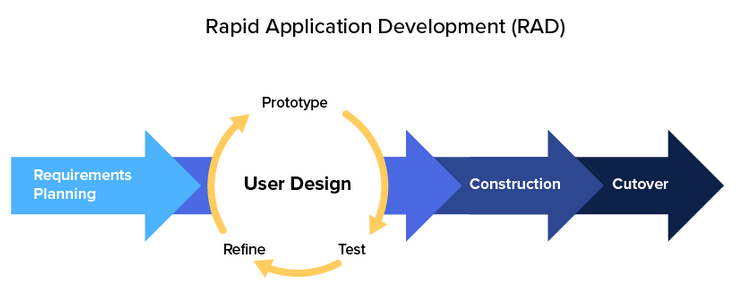
\includegraphics[width=\textwidth]{images/misc/RAD.png}
	\captionsource{Etapas que componen la metodología RAD}{\cite{kissflow_2018}}
	\label{fig:rad}
\end{figure}

\subsection{Herramientas de desarrollo}

El hardware a ser utilizado para el desarrollo de la solución corresponde al siguiente:
\begin{itemize}
    \item Notebook Acer Aspire E5-575G, CPU Intel Core i5-6200U, 8GB memoria RAM, GPU NVIDIA GeForce 940 MX, 1GB VRAM.
    \item Dos cámaras USB Webcam Logitech HD Pro C920 1080p Widescreen.
    \item Sensor de gestos de manos Leap Motion.
    \item Mini Proyector Led Full HD 1080p, 1200 Lúmenes, Unic UC46.
    \item Dispositivo \textit{eye tracking} Tobii o Eyetribe.
\end{itemize}   

En términos del software a ser utilizado, se encuentran las siguientes herramientas:
\begin{itemize}
    \item Visual Studio Community 2019
    \item Sistema Operativo Windows 10
\end{itemize}

\section{Organizaci\'on del documento}
\label{intro:organizacion}

